\documentclass[journal,12pt,onecolumn,draftclsnofoot,]{IEEEtran}
\IEEEoverridecommandlockouts
% The preceding line is only needed to identify funding in the first footnote. If that is unneeded, please comment it out.
\usepackage{cite}
\usepackage{amsmath,amssymb,amsfonts}
\usepackage{algorithmic}
\usepackage{graphicx}
\usepackage{textcomp}
\usepackage{xcolor}
\usepackage{url}
\usepackage{listings}
\def\BibTeX{{\rm B\kern-.05em{\sc i\kern-.025em b}\kern-.08em
    T\kern-.1667em\lower.7ex\hbox{E}\kern-.125emX}}
\begin{document}

\title{The Halting Problem}

\author{
\IEEEauthorblockN{Holly McCoy, Grant Gurvis, Ali Bayatpoor}

\IEEEauthorblockA{\textit{Computer Science and Engineering} \\
\textit{University of South Florida}\\
Tampa, Florida \\
ggurvis@usf.edu}
}

\maketitle

\begin{abstract}
  The Halting problem is one of the most famous undecidable problems in math and computer 
  science, an introduction to it will be given along with proof of why it is not decidable.
  Lastly, a program will be explained that can show whether very small Turing machines halt.
\end{abstract}

\begin{IEEEkeywords}
automata, formal languages
\end{IEEEkeywords}

\section{Introduction}

The Halting Problem is an issue in computer science which refers to the inability of a computer program to effectively and definitively declare whether a program halts or infinitely loops. Computer scientists have deemed this problem as being an “undecidable” problem, which means it is impossible to solve, and it can never be solved. In this paper we will be investigating what exactly the halting problem is, how one could theoretically solve the problem (though it can never be implemented in actuality), a mathematical proof by contradiction proving that the problem is unsolvable, and some concluding remarks highlighting the importance of the issue. 

\section{Halting Problem}

Let us consider what exactly is defined as a “halt” in a program, and what is defined as an “infinite loop” in a program. Take for example a simple Hello World program, in which all that is contained in the program is a print statement that says \verb|print("Hello World")|. Once the program runs, the string will be printed to the output and the program will automatically halt upon execution, thus describing what a “halt” looks like in a program. Now take for example a program with the following code: 

\begin{lstlisting}[language=Python]  
x = 1 

while x == 1: 
  print("Hello World")
\end{lstlisting}

The variable \verb|x| was initialized to equal one, and the loop is commanded to run so long as \verb|x| equals one. The value of \verb|x| is never changed, so the loop will run infinitely until it is forcibly terminated by the developer, thus demonstrating an infinite loop. 

To get a better understanding of the complexity of the problem, we will now introduce a theoretical algorithm which should solve the halting problem in theory, yet it cannot be implemented in actuality. While the purported solution is by no means a true solution, it will serve to paint a better picture of what exactly the halting problem is, the complexity associated with it, and why it is ultimately an unsolvable problem. Suppose there is a program called “The Decider” which takes in two inputs; namely, another program which we will call “ProgramX” along with some intended input for ProgramX which we will call “InputX”. Ideally, we want the Decider to declare to us, upon taking in ProgramX and InputX, whether ProgramX halts, or infinitely loops after reading InputX. If ProgramX halts upon reading InputX, the output of the Decider should be “Halt”. If ProgramX infinitely loops upon reading InputX, the output of the Decider should be “Loops”.  

Now we will investigate the problems associated with the proposed algorithm. The first problem lies in determining how long the Decider is to wait to declare if the program halts or loops upon processing InputX into ProgramX. Should it wait 60 seconds, 60 minutes, 60 hours, or even 60 days if the program still has not halted? How much time defines whether a program infinitely loops or not? You would need more than an infinite amount of time for that. An infinite loop never stops, so how can we define whether a loop is infinite or not since we do not know if the program may just need more time to halt? Suppose the program halts after 12 seconds, then the correct output can be shown by the Decider, and it would display the string “Halt” to the output. But if the program infinitely loops, the Decider will be waiting an infinite amount of time to figure that out, and so it will never actually display “Loops” to the output. Therefore, the proposed algorithm cannot solve the halting problem even though in theory it should, so to definitively prove that the halting problem is unsolvable, let us use a proof by contradiction. 

\subsection{Proof}

Assume that there is a machine (H) that solves the halting problem, H can be fed the logic of another machine (X) such that the output of H will always accurately be whether machine X  will loop infinitely or halt when fed itself. 

Let X’s 2 cases show: 
\begin{center}
  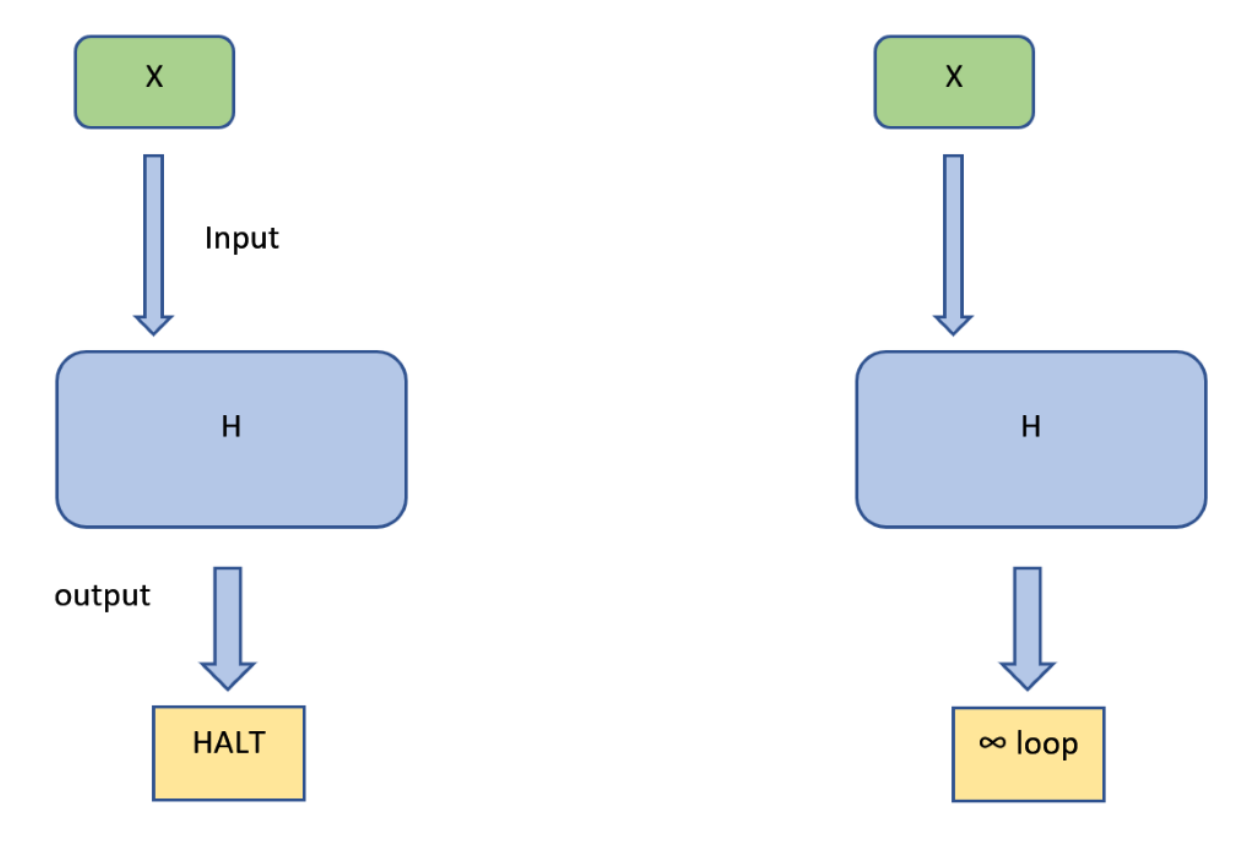
\includegraphics[scale=0.3]{1}
\end{center} 

Now assume machine Y can be fed H and will always do the opposite of H’s output such that: 

 
\begin{center}
  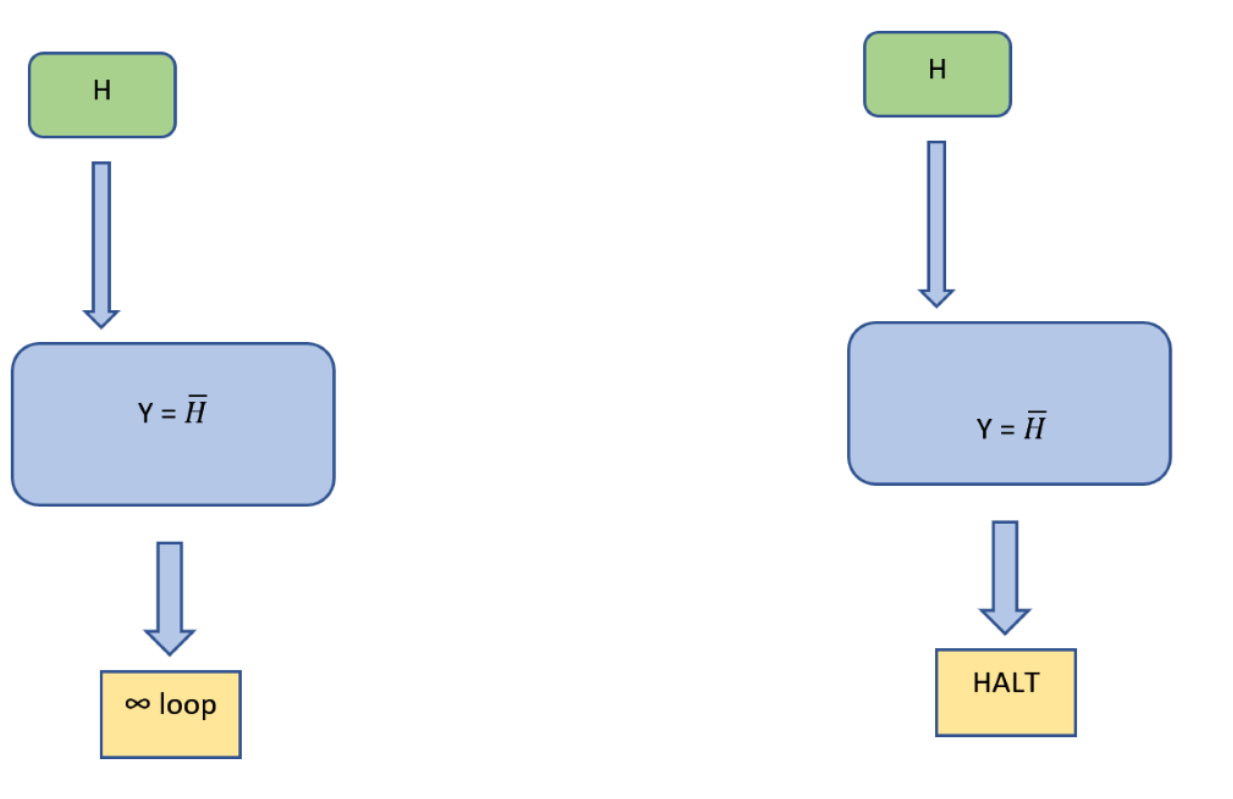
\includegraphics[scale=0.3]{2}
\end{center} 

Then If we use Y a/s an input for H we will run into a contradiction that whatever H’s output is, will be the incorrect answer as Y is the complement of H: (visual below for logic) 

\begin{center}
  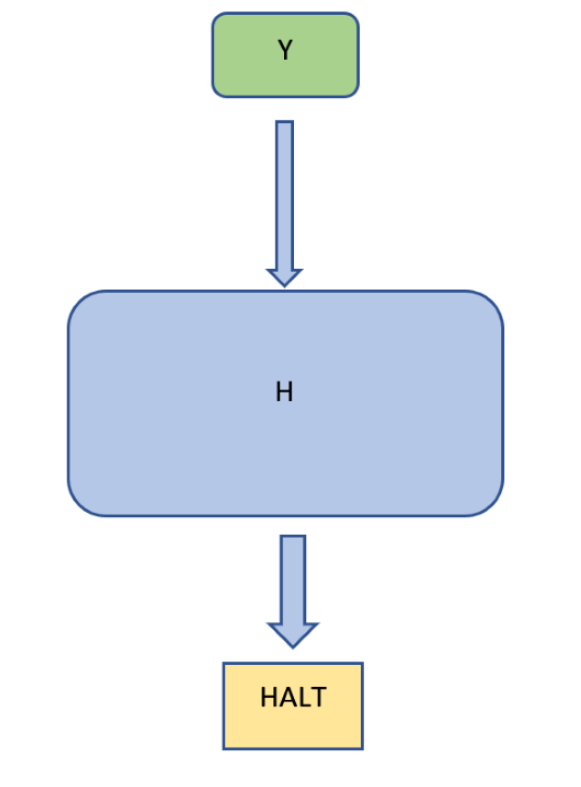
\includegraphics[scale=0.3]{3}
\end{center} 

Because H’s result is a halt, Y’s answer should be an infinite loop because Y =  , meaning H could not accurately express the result of Y hence by contradiction H does not solve the halting problem

\section{Practical Example}

Using the knowledge that for any arbitrary TM the result of if it halts or not is not
determinable a program can be constructed that shows that a small subset of Turing machines
can be shown to halt or not and the limiting factor on this. First an encoding of Turing 
machines will be shown, this will allow the program to be consistent and easily enumerate 
over all Turing machines of $n$ states and $m$ symbols.

\subsection{Turing Machine Enumeration}

To enumerate over the set of machines there needs to be a way to identify a specific
Turing machine, to do this a \textit{descriptive number} will be used that will encode
each machine as a string of letters.~\cite{computable_numbers}

For each Turing machine the machine will be described by a string with each transition being
described in the format \verb|Symbol-Shift-State|, the string for the 3-state 
2-symbol 
busy beaver would be: 

\begin{center}
  {\verb|3-2/1-1-2/0-1-3/1-0-3/1-1-0/1-1-2/1-0-1|}
\end{center}

Each transition 
function is separated by a \verb|/|. At the beginning is the number of non-halting states than the number
of symbols so the encoding is not ambiguous for cases where there are the number of transitions
are equal but the states and symbols are not. There is only one halting 
state which any function can transition to, but it does not count in the size of the transition
function so a 3-state description is actually a 4-state Turing machine with 3 non-halting
states that can transition to the halting state depending on the encoding. For the encoding
the 0 state is the halting state, 0 is left, and 1 is right. Using this description of a 
Turing machine every Turing machine of $n$ total states, $h$ halting states, and $m$ symbols
can be constructed, where $h = 1$. The encoding can also be easily enumerated over allowing 
for each encoding to be given a number from 0 to ${(2nm)}^{(n-h)m}$. This numeric encoding
is similar to Gödel numbering but it is unique to each n-state Turing machine for the 
simplicity of this program.

\subsection{Busy Beaver}

The Busy Beaver simply put the Turing machine with $n$ states and $m$ symbols that takes the 
most number of steps of any other Turing machine with similar states and symbols while still 
halting, sometimes also looked at as the Turing machine
which produces the most tape output but when it comes to the halting problem the step
perspective is more pertinent. Since the number of symbols in a Turing machine does not
increase its power only the situation with 2 symbols will be focused on. The Busy Beaver
TM for $n$ states performs $S(n)$ steps which is the most number of steps that a finite $n$ 
state TM can take. Using this knowledge all that a TM needs to be done to prove that it
halts is run it for $S(n)$ steps and it can be concluded either it halts or does not.
This unfortunately does not actually solve the Halting problem though as finding a 
Busy Beaver for $n$ is not computable.~\cite{rado} Only the first 4 $n$ are known, 1=1,
2=6, 3=21,
and 4 = 107.~\cite{oeis} The Busy Beaver function is very interesting as it is the fastest
growing function which even out classes the ability to be computed. The current know limit on
the computation of the function is $n=1919$ which if computed would violate the 
Zermelo-Frankel set theory.~\cite{8000}\cite{1919} This gives the situation of there being finite numbers 
that is not computable.

\subsection{Program}

However since these small $n$ are known a program can be made to show how the $S(n)$ function
could solve the Halting problem, in fact for Turing machines with 4 or less non halting states
and 2 symbols it can be shown if a Turing machine will halt or not given the busy beaver. 
To do this first the busy beaver transition functions are encoded in the aforementioned 
encoding scheme, as well as some lower bounds for 5 and 6 states since they could be 
the busy beaver but are unproven. The Turing machines come from various papers but are 
collected by the Busy Beaver Competition which tracks the best attempts at finding busy
beavers for n-state turing machines.\cite{comp}
Next the busy beaver function is run and the number of steps
is counted. Finally a second Turing machine that is being tested to be determined if it halts
is run and either halts or is stopped when it reaches the number of steps that the busy beaver
ran for. It is then shown that the Turing machine halts or will never halt. This program is
in Python and allows for random, number encoded, and transition encoded Turing machines
to be run.~\cite{halting-prog}

\section{Conclusion}

Being able to solve the halting problem would have some major implications in math, for 
example there are Turing machines that will halt/not halt iff ZFC is inconsistent, the 
Riemann hypothesis is false, or iff Goldbach's conjecture is false.\cite{1919}
If these Turing machines
could be shown to be halting or not it would allow for major mathematical discoveries and 
proofs. The halting problem would also be more directly relevant to a programmer who need to 
verify systems work as expected and will either end or loop forever. Continuing to attempt
to solve the halting problem for a larger range of machines will advance both math and 
computer science such even a minor breakthrough in the complexity of analyzing these 
machines would allow for the possibility major breakthroughs in other areas.

\bibliographystyle{IEEEtran}
\bibliography{report}

\end{document}


